\setcounter{chapter}{5}
\chapter{Milestones}
In this chapter, we describe the phases of our plan for exploring the research challenges and investigating the research issues identified in Chapter 4. This chapter also includes research methodology and future publication plan.

\section {Research Methodology and Time Line}

    \par The goal of the research project of my Ph.D program is to propose a technically and economically feasible architecture for path stability in MANETs environment.

    \begin{figure}
                \begin{center}
                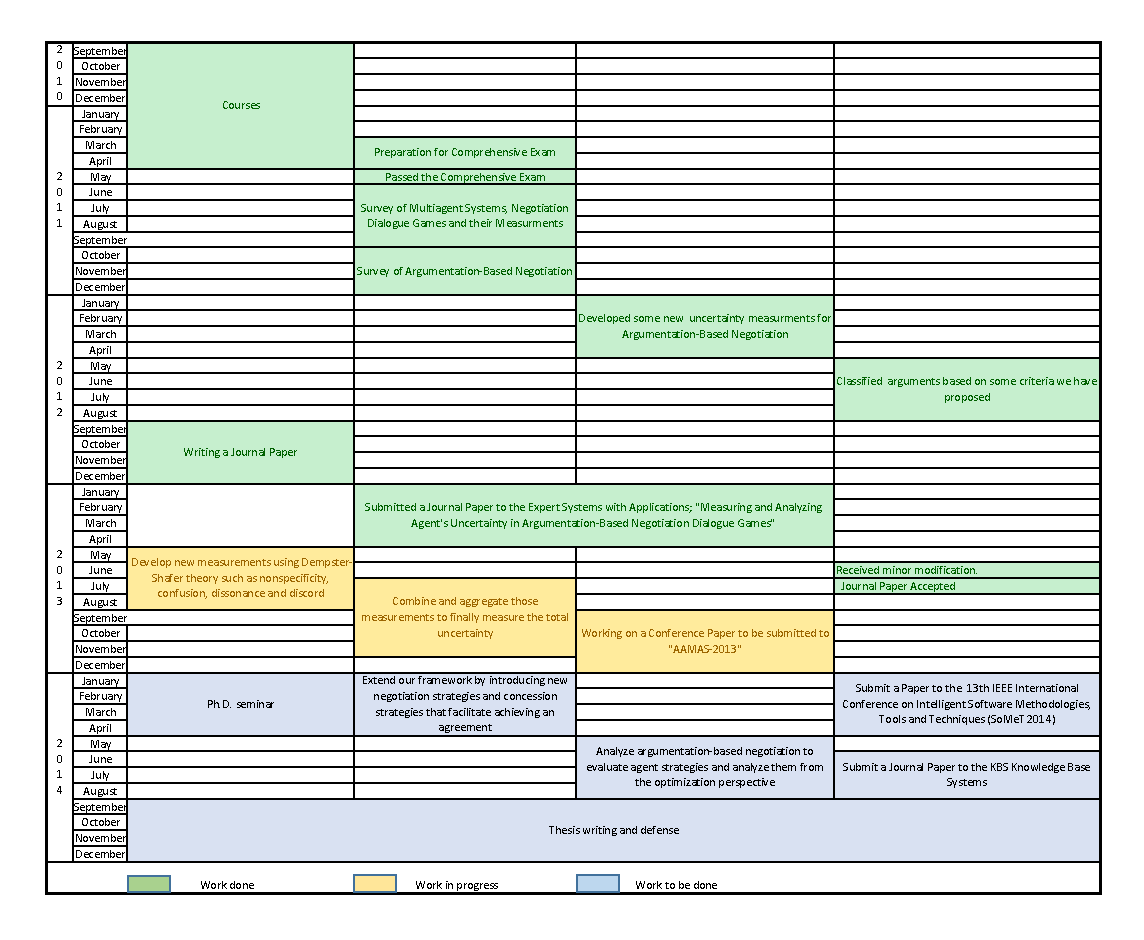
\includegraphics[width=16cm, height=22cm]{Figures/timetable.eps}\label{Timetable}
                \caption{Research milestones and time line}
                \end{center}
\end{figure}

   % To investigate the architecture of MANETs, we will experiment on backup path, protection, transmission range, interference, and multi Path modeling and analysis on 3D MANETs technologies. We will apply an efficient clustering algorithm for the hierarchical placement of equipment in the above mentioned access network architecture. We will develop mathematical models for different architectures. We will also investigate the protection schemes for these architectures.



The time duration of each task includes the modeling of the proposed solution,  its implementation, validation, performance evaluation  and  publication of its outcome.

\section {Publication Plan} 